%%%%%%%%%%%%%%%%%%%%%%%%%%% Paper.tex %%%%%%%%%%%%%%%%%%%%%%%%%%%%%%%
% Template for producing ASME-format journal articles using LaTeX    %
% Written by   Harry H. Cheng, Professor and Director                %
%              Integration Engineering Laboratory                    %
%              Department of Mechanical and Aeronautical Engineering %
%              University of California                              %
%              Davis, CA 95616                                       %
%              Tel: (530) 752-5020 (office)                          %
%                   (530) 752-1028 (lab)                             %
%              Fax: (530) 752-4158                                   %
%              Email: hhcheng@ucdavis.edu                            %
%              WWW:   http://iel.ucdavis.edu/people/cheng.html       %
%              May 7, 1994                                           %
% Modified: February 16, 2001 by Harry H. Cheng                      %
% Modified: January  01, 2003 by Geoffrey R. Shiflett                %
% Use at your own risk, send complaints to /dev/null                 %
%%%%%%%%%%%%%%%%%%%%%%%%%%%%%%%%%%%%%%%%%%%%%%%%%%%%%%%%%%%%%%%%%%%%%%

%%% use twocolumn and 10pt options with the asme2e format
\documentclass[twocolumn,10pt]{asme2e}

\makeatletter
\let\asme@citex\@citex % save amse2e definition of \@citex
\makeatother

\usepackage{textcomp}
\usepackage[USenglish]{babel}    % English

\makeatletter
\let\@citex\asme@citex % restore
\makeatother
\usepackage{float}
\usepackage[ansinew]{inputenc}   % Output glyphs like 'ö' at all
%\usepackage[T1]{fontenc}        % Output glyphs like 'ö' in a nice font
\usepackage{graphicx}            % For loading graphic files
%\usepackage{a4wide}             % Smaller margins = more text per page.
\usepackage{fancyhdr}            % Fancy headings
\usepackage{longtable}           % For tables, that exceed one page
\usepackage{xspace}              % Geeft spaties na commando's die dat behoeven
%\usepackage{titling}
\usepackage{standalone}
\usepackage{subcaption}

\usepackage{mathtools}             % Math packages
\let\proof\relax 
\let\endproof\relax
\usepackage{amsthm}
\usepackage{amsfonts}
\usepackage{fancyhdr} 
\fancyhf{}
\cfoot{\thepage}
\pagestyle{fancy}    

%% The class has several options
%  onecolumn/twocolumn - format for one or two columns per page
%  10pt/11pt/12pt - use 10, 11, or 12 point font
%  oneside/twoside - format for oneside/twosided printing
%  final/draft - format for final/draft copy
%  cleanfoot - take out copyright info in footer leave page number
%  cleanhead - take out the conference banner on the title page
%  titlepage/notitlepage - put in titlepage or leave out titlepage
%  
%% The default is oneside, onecolumn, 10pt, final


\title{Determining Tire Characteristics Through Data Driven Modeling}

%%% first author
\author{Eugene Figueiras
    \affiliation{
	BSC student\\
	TU Delft\\
    SN:4257669 
    }	
}

%%% second author
%%% remove the following entry for single author papers
%%% add more entries for additional authors
\author{Maarten Kleijwegt
    \affiliation{
	BSC student\\
	TU Delft\\
    SN:4113810 
    }	
}

%%% third author
%%% remove the following entry for single author papers
%%% add more entries for additional authors
\author{Nol R{\"o}mer
    \affiliation{
	BSC student\\
	TU Delft\\
    SN: 4391888
    }	
}

\author{Akash Soerdjbalie
    \affiliation{
	BSC student\\
	TU Delft\\
    SN: 4227174
    }	
}

\begin{document}

\maketitle    

\begin{abstract}
\textbf{\textit{Abstract} - With the use of Nonlinear Model Predictive Control (NMPC), it could become possible for autonomous driving systems to operate passenger cars at the limits of handling, which could help prevent accidents. In order to achieve NMPC, a valid model of the dynamic behaviour of a vehicle is essential. This paper describes how a model of the tire characteristics of a vehicle is designed, using a sensor-equipped scaled RC car. In order to do so, many characteristics of the dynamics of the car are measured. Using those data and the Bicycle Model, the slip angles, slip ratios and tire forces are calculated. Afterwards, the tire characteristics are modeled using the Magic Formula. This method proves to be a useful approach, but due to some minor errors in the test data, only a part of the tire characteristics could be determined.}
\end{abstract}
\section{Introduction}
In the United States alone, the National Highway Traffic Safety Administration \cite{NHTSA} reports that traffic accidents have taken 37,000 lives in 2016. Until now, driver safety systems in modern cars have focused on keeping the friction of the tires of cars in the linear regime while driving. For example, ABS prevents the wheels from locking and traction control prevents the car from losing grip on the road. However, when we look towards professional rally drivers, we see that operating in the linear regime is not specifically necessary for driving safely. If cars were to operate safely in the nonlinear regime of friction, more accidents can be prevented. It would give Driver Aid Systems more capabilities and options. This might result in better accident prevention solutions.

This project focuses on establishing a measurement setup and determining the tire characteristics of a small-scale RC car with it. It is a step towards developing a correct Nonlinear Model Predictive Control (NMPC) system that enables autonomous driving on the limits of handling. NMPC is a control method which uses a dynamical model that can predict the motion of the car. Therefore, this system is able to let the car make evasive maneuvers up to and including the nonlinear regime of driving \cite{Tamas}. In order to obtain a correct dynamical model for the NMPC, tire characteristics are required.

There are a few ways to obtain these tire characteristics. Usually, they are determined using special test rigs in which only the wheels are placed. However, these test rigs are very expensive and the characteristics are only valid for the given tire, in only the given condition (think of temperature, state and wetness of the tire) on only a single given surface \cite{Jonson}. A lot of testing can be done to determine the characteristics of all tires in all conditions. Yet it could be far better if a car would be able to determine its own characteristics using on board sensors such as GPS and Inertial Measurement Units (IMU). Testing with real cars and on-board sensors in a special test environment is a possibility, but developing and refining this technique on small scale RC cars first requires less resources such as large test tracks and expensive cars and tires. Therefore, using a small-scale RC car equipped with sensors is by far the least expensive way to obtain these tire characteristics. When proven successful, these methods can then be applied on actual cars to determine their tire characteristics.

This paper strives to determine the tire characteristics of a small scale RC car using only on board sensors and a motion capture system that represents GPS-type information. Section 2 discusses some scientific background on the topic. After this, the experimental setup and data processing will be explained in Section 3. Next, in Section 4, results will be discussed. Finally, the conclusions will be given in Section 5. The paper also leaves some room for recommendations and acknowledgements.  


\begin{figure*}
	\centering
		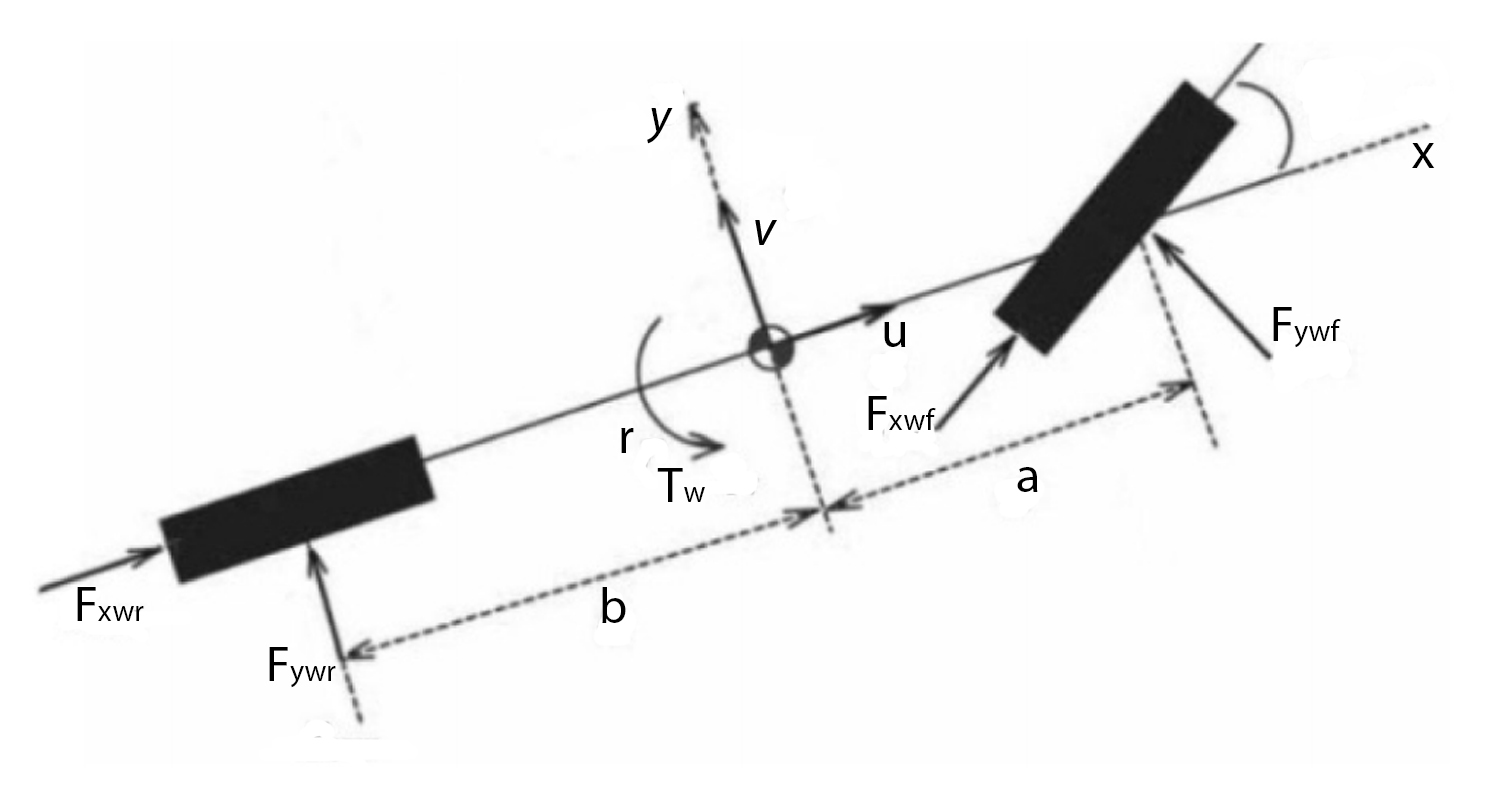
\includegraphics[scale=0.34]{figure/bicyclemodel.jpg}
	\caption{Bicycle model}
    \label{fig:bicyclemodel}
\end{figure*}

\section{Modelling}
In order to determine the tire characteristics with a measurement setup, it is important to use a vehicle model to describe the dynamics of the RC car. Furthermore, the tire characteristics will be described with a model as well. This section describes the vehicle and tire model used in this setup. 

\subsection{The Bicycle Model}
The model used to describe the behavior of the RC Car is the 3 DOF Bicycle Model (Figure \ref{fig:bicyclemodel}) \cite{Liu}. This model consist of the longitudinal (x), lateral (y) and yaw ($\psi$) motion. This model considers that the mass of the vehicle is entirely in the rigid body of the base. Load transfer due to pitch/roll were neglected. This means there is a constant normal force (F\textsubscript{z})  on the wheels. The equations that describe the motion of this model are described as follows:

\begin{subequations}
\begin{align}
    m(\dot{u}-vr) = \sum F_{xi} \quad   (i= f,r) \\
    m(\dot{v}+ur) = \sum F_{yi} \quad   (i= f,r) \\
	I_{z}\dot{r} = F_{yf}a - F_{yr}b\\
	r = \dot{\psi}
    \label{eq:motion}
    \end{align}
\end{subequations}

The longitudinal force (F\textsubscript{xi}) and lateral force (F\textsubscript{yi}) act along the x and y-axis, respectively. The relationship between these forces and the orientation of the wheels are given by equations \ref{eq:bicycle}

\begin{subequations}\label{eq:bicycle}
\begin{align}
	F_{xi} = F_{xwi}\cos\delta_{i}-F_{ywi}\sin\delta_{i} \quad (i=f,r)\\
	F_{yi} = F_{xwi}\sin\delta_{i}+F_{ywi}\sin\delta_{i} \quad (i=f,r)
	\end{align}
\end{subequations}

Where F\textsubscript{xwi} is the longitudinal tire force and F\textsubscript{ywi} is the lateral tire force. 

The difference between the speed of the RC Car and the angular velocity of the wheel is given as a ratio by equation:

\begin{subequations}
\begin{align}
	\kappa =1-\frac{u_{wi}}{R_{w}\omega_{wi}} \quad u_{wi}\leq  R_{w}\omega_{wi} \quad (acceleration)\\
	\kappa = \frac{R_{w}\omega_{wi}}{u_{wi}} -1 \quad u_{wi}> R_{w}\omega_{wi} \quad (Braking)
	\label{eq:kappa}
\end{align}
\end{subequations}

This equation is known as the \textbf{longitudinal slip ratio}, where R\textsubscript{w} stands for the radius of the wheels and $\omega$\textsubscript{wi} for the angular velocity of the wheels. The following equations are used to calculate the  slip angle, where $\alpha\textsubscript{f}$ and $\alpha\textsubscript{r}$ are the \textbf{slip angles} for the front and rear tires, respectively. 
\begin{subequations}
\begin{align}
    \label{eq:alpha1}
	\alpha_{f} = \delta_{f}-\frac{v+ar}{u_{wf}}\\
	\alpha_{r} = \frac{br-v}{u_{wr}}
	\label{eq:alpha2}
\end{align}
\end{subequations}



\subsection{The Magic Formula}	
%eerste zin moet nog iets anders
Since it is necessary to know how the tires would behave in a combined slip condition, not all tire models are suitable. Three models that are able to model this behavior  are: The Dugoff model,The Brush Model and The Magic Formula of Pacejka \cite{Pacejka}. The model used in this experiment is the Magic Formula of Pacejka (Figure \ref{fig:MagicFit}). This semi-empirical model is the most accurate of these three. Another major advantage of this model is that it is described by one single equation. The Dugoff model and the Brush model use separate equations for the linear and non-linear regime, which is a major drawback due to the difficulty in determining at which moment at which region the car is operating \cite{uil}.The general Magic Formula has the following form:

\begin{equation}
	y = D\sin (Ctan^{-1}(Bx-E(Bx-tan^{-1}(Bx)))) \quad
    \label{eq:magicf}
\end{equation}

This equation is valid in the case of pure longitudinal slip or in the case of pure lateral slip. In the case of pure longitudinal slip y is replaced with F\textsubscript{x} and x is replaced with $\kappa$. In the case of pure lateral slip y is replaced with F\textsubscript{y} and x with $\alpha$. The data of y and x are measured and the variables B,C,D, and E are used to fit the formula to the data.

When combined slip occurs the formula changes to:
\begin{subequations}
\begin{align}
\begin{split}
F_{x}&=\cos(C_{x\alpha}\tan^{-1}(B_{x\alpha}tan\alpha))\\
& \quad *D_{x}\sin(C_{x}tan^{-1}tan(B_{x}\kappa-E_{x}(B_{x}\kappa-tan^{-1}(B_{x}\kappa)))\\
\end{split} \label{eqmagiccombined1}\\
\begin{split}
F_{y}&=\cos(C_{y\kappa}tan^{-1}(B_{y\kappa}\kappa))\\
& \quad *D_{y}*sin(C_{y}tan^{-1}(B_{y}\tan\alpha\\
& \quad -E_{y}(B_{y}\tan\alpha-\arctan(B_{y}\tan\alpha))))\\
\end{split} \label{eq:magiccombined2}
\end{align}
\end{subequations}


\begin{figure}[h!]
	\centering
		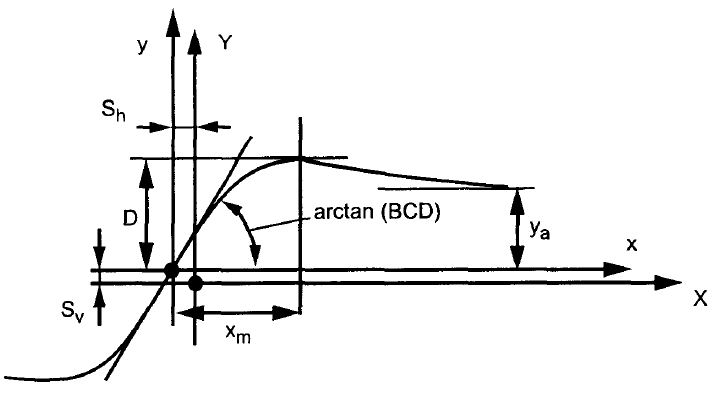
\includegraphics[scale=0.4]{figure/Magic_Formula.png}
	\caption{ Pacejka Magic Formula for tire modeling}
    	\label{fig:MagicFit}
\end{figure}

\section{Experimental setup}
 
In order to determine the tire characteristics of the scaled vehicle, a good testbed is necessary. In this section, the experimental setup used to gather the data needed for determining the tire characteristic is discussed. As concluded from the model, the following variables are required to measure the tire characteristics: 
\begin{itemize}
	\item$\bullet$ linear accelerations of the car
    \item$\bullet$ linear and angular velocities of the car
    \item$\bullet$ steering angle of the front wheels
    \item$\bullet$ angular velocities of the wheels
\end{itemize}
The experimental setup consists of a modified scaled RC car with an on board IMU, feedback servo and a tachometer on each wheel. Moreover, a motion capture system, or MoCap, was used to provide millimeter precision localization. The IMU is used to measure the velocities and accelerations of the car. The feedback from the servo is used to determine the steering angle. The tachometers are used to measure the angular velocity of the wheels. The MoCap was used to check and calibrate the signal coming from the IMU. However, the noise on the MoCap location signal, which is amplified by differentiation, made it unfit for this research.

\subsection{Car}
The RC car is a Losi TEN Rally-X. It is a 1:10 scale car with 4WD powered by a 2s 6000 mAh LiPo battery and a 3900 KV Fuze Brushless DC motor. With this battery the car is able drive at speeds between 1.5 and 15 m/s.  To meet the assumptions of the Bicycle model, the suspension of the car was replaced with stiff turnbuckle rods to eliminate the degrees of freedom of roll and pitch. The wheels are custom 3D-printed rims with grip tape applied to simulate tires and fitted with 2 magnets each. When the magnets pass a hall-effect sensor on the car a signal is created of 2 pulses per revolution. The hall-effect sensors and the magnets make up the tachometers of the car. Another set of wheels with space for 24 magnets was created, but due to lack of time, no tests were conducted with these. The IMU was mounted in the center of gravity of the car, preventing angular velocities from influencing the accelerometer. Finally, the standard servomotor was replaced by a robot servomotor, which allowed for reading the angle from the servomotor angle sensor.

\subsubsection{MoCap}
The MoCap is used as a positioning system. A MoCap system cannot be regarded as an on-board sensor, as it requires an area with aligned cameras. However, in this case it is used as a replacement for a GPS sensor. The MoCap system enables us to do testing inside, something which is not possible with a GPS system. Finally, the MoCap system was ready to use and already connected with ROS, using a sampling rate of 120 Hz.

\begin{figure*}
  \centering
    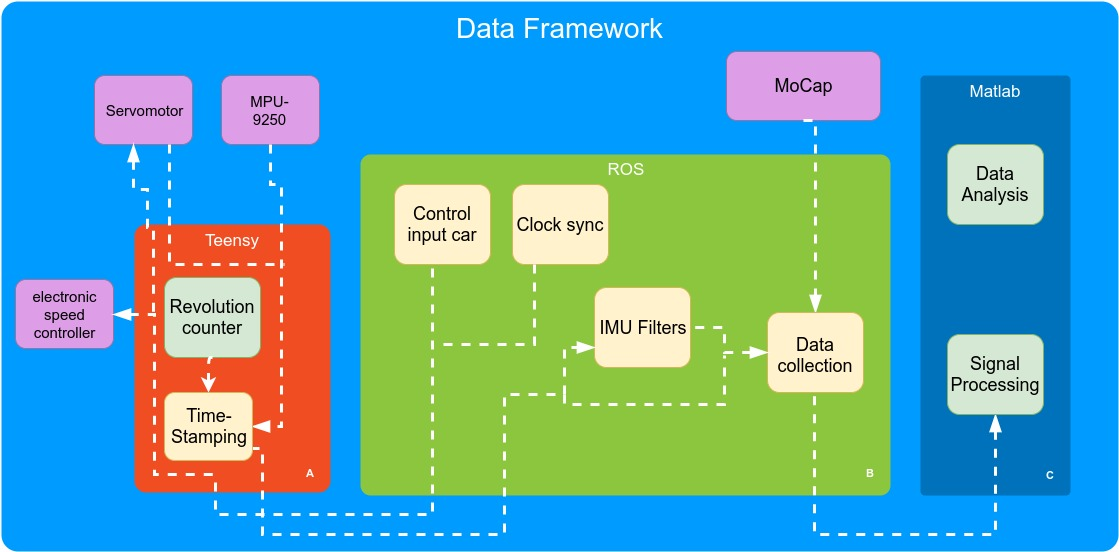
\includegraphics[scale=0.40]{figure/DataFramework__1_.jpg}
  \caption{Data acquisition framework}
  \label{fig:DonutFramework} 
\end{figure*}

\subsection{Data acquisition and processing}
Data acquisition was done using a ROS (Robot Operating System) based system. The sensors were connected to a Teensy 3.6 prototyping board running a custom ROSserial node, connected to a Raspberry Pi 3 model B running ROS. The custom ROSserial node uses an interrupt controlled program to gather sensor data in a fast and accurate way. Moreover, on-board hardware timers were employed as pulse counters for the tachometer-signal.
The MoCap is connected to the system utilizing the labs Wi-Fi network. Further communication was done using a self-written ROS package. After data collection, further processing was done using Matlab. Figure
\ref{fig:DonutFramework} further elaborates the Data acquisition framework.

\subsubsection{ROS}
Implementing ROS on the testbed provided it with some key components needed for accurate testing. Since ROS has already been established as a research and prototyping framework, a lot of packages are already developed for this operating system and are easily available.  One key component is timestamping. To provide usable data, the testbed needs a timestamping method. ROS automatically syncs all the clocks on every device providing a convenient solution to this problem. Furthermore, our testbed contains a simple IMU which does not provide all data that a more advanced IMU might offer, like orientation or sensor fusion between the magnetometer and gyroscope signal. Therefore a complementary filter was used in ROS to generate this data. \cite{IMUfilter}. The complementary filter was chosen for this purpose as its transfer function and implementation is the same as a Kalman filter. However the complementary filter has improved response time. Moreover, the MoCap generated its data already in ROS, which meant combining everything in ROS would be a simplification. Also, ROS offers convenient data recording options called ROSbags, which can be imported into MATLAB for further analysis.

\subsubsection{Sampling}
The sampling rate for our experiments was set at 120 Hz. The MoCap already operated at this sampling rate and to simplify synchronizing our data points one sampling rate was used. Moreover, if all sensors would work on the same sampling rate, this would reduce the hardware requirements on the Teensy and reduce the need for data interpolating. 

Since a lot of noise was apparent on the IMU signal in initial tests, the decision was made to employ the built-in Digital Low Pass Filter (DLPF) on the IMU, to decrease noise and data rate at the same time. However, this would create a delay on our signal. To prevent this delay from becoming significant, a limit of 10ms signal delay was chosen. A 92 Hz DLPF was chosen since it only created a delay of 7.8 ms, but would decrease the data rate significantly without losing data points. To prevent signal aliasing, a sampling rate of 92 Hz or higher is required. Our sampling rate of 120 Hz fills this requirement

% Since the MoCap already delivered her data at a sampling rate of 120 Hz, it was easy to pick this as the target sampling rate for the whole system. Because initial tests showed no accelerations beyond 1.5 g, this would mean the maximum increase of velocity per timestep would be 0.122[m/s]. This was deemed accurate enough for this research. Moreover, testing will also be done at speeds as slow as 1.5[m/s], including accelerating from standstill. With 24 magnets this would result in signals of 127 Hz. If the sampling frequency would be higher than the frequency of wheel pulses, this would generate multiple points with the same distance traveled, as no new pulses from the wheel were encountered in between. This increases signal analysis difficulty requiring further interpolation before analysis can be done. Since the goal was always to use 24 magnets per wheel, this sampling rate was used from the beginning. Moreover, 2 magnets would create a signal with a frequency of only 10.6 Hz. As a sampling frequency of 10 Hz or even lower has a resolution of only 0.1 s, in which a pulse could have been generated at any given time, this was deemed too low so the sampling rate was kept at 120 Hz. Furthermore, the IMU generates data at sampling rates reaching 1000 Hz. Testing showed however, that ROS was only capable of reaching speeds of 300Hz on the Raspberry Pi. Moreover, since a lot of noise was apparent in initial tests, the decision was made to employ the built-in Digital Low Pass Filter(DLPF) to decrease noise and data rate at the same time. However, this would create a delay on our signal. To prevent this delay from becoming significant, a limit of 10ms signal delay was chosen. A 92 Hz DLPF was chosen since it only created a delay of 7.8 ms, but this decreased the data rate significantly without losing data points. To prevent aliasing, a sampling rate of 92 Hz or higher was needed. This made it possible to have all the sensors to work on the same sampling rate to reduce hardware requirements on the Teensy and reduce data interpolating. 

\subsubsection{Experiments}
The experiments can be classified into three groups.

The first set of experiments is carried out in a straight line (longitudinal motion). During these experiments, the car accelerated and braked while driving straight ahead. 

The second set consists of the steady state cornering experiments (lateral motion). Steady state cornering means cornering at a constant longitudinal velocity and constant steering angle. 

Finally, the third set of experiments take both lateral and longitudinal motion into account. Variables of the tests are acceleration/deceleration for longitudinal motion, longitudinal velocity and steering angle for lateral motion, and these three combined for combined motion. The variables were slightly increased in each experiment in order to determine the transition from linear to nonlinear behaviour.

\subsection{Data filter} 	
The experimental data is collected in ROSbags and processed afterwards. This makes it possible to filter the noise from the IMU with a Zero-Phase Low Pass Butterworth Filter. This is a non-causal filter with a phase slope of zero which eliminates any delay that is commonly caused by causal filters. The Low Pass filter is of the 20th order, in order to approach an ideal Brick wall Response, with a cut-off frequency of 5Hz. A Fourier spectrum analysis was done, however the signal from the IMU was indistinguishable from the noise. Therefore, it was reasoned most of the noise would be from vibrations generated by the wheels and at the minimal speed of 1.5 m/s these would rotate at 5.3 Hz. Therefore a "Brick wall" response, as seen in figure (\ref{fig:brickwall}) at 5 Hz was selected. This would cancel out most of the noise, but keeps most of the signal intact. 
	\begin{figure}
	\centering
	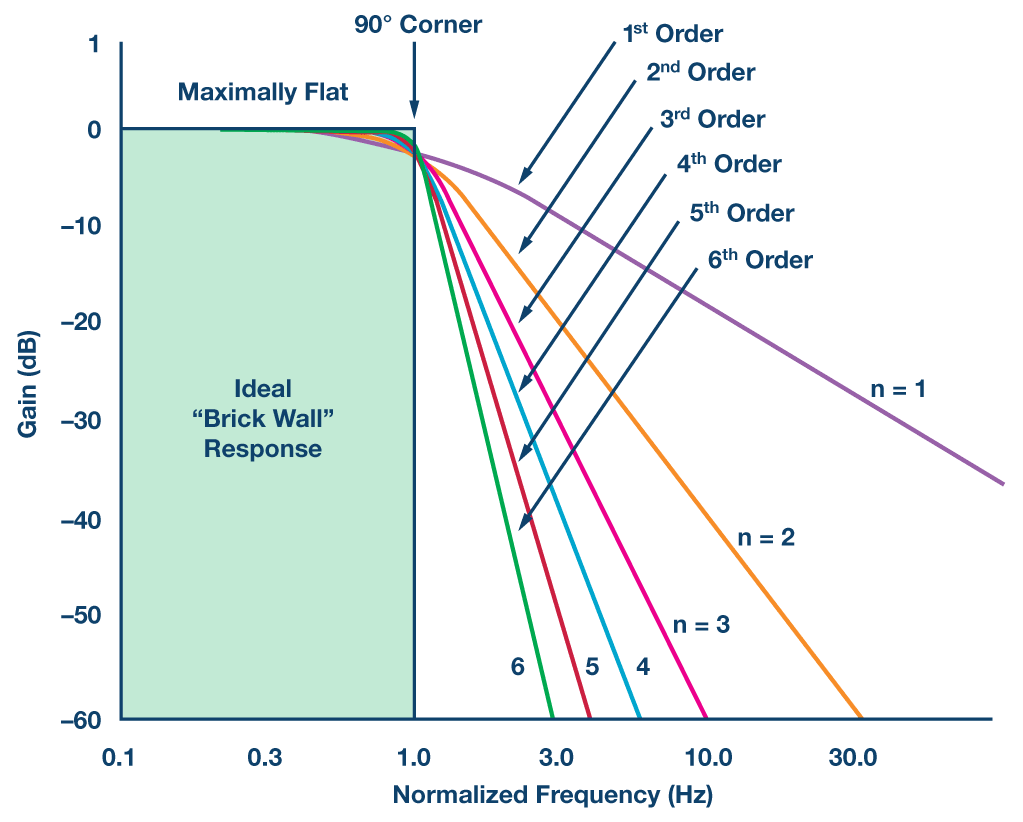
\includegraphics[scale=0.17]{figure/brickwall.png}
	\caption{Brick wall response}
	%\captionsource{Caption}{(http://www.electronics-tutorials.ws/filter/filter_8.html)}
	\label{fig:brickwall}
	\end{figure}






\section{Results and discussion}

\begin{figure*}
	\centering
	\begin{subfigure}{1\linewidth}
		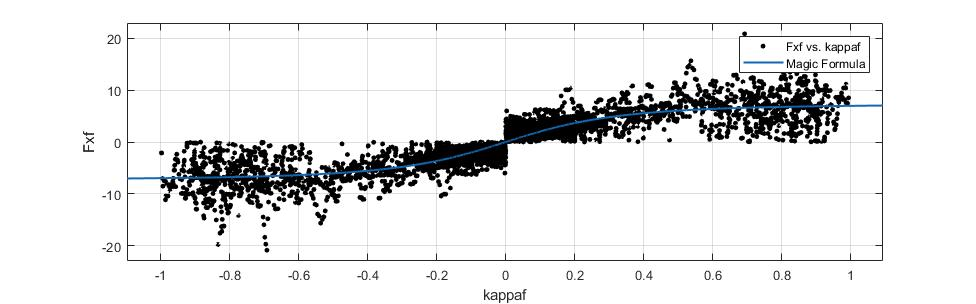
\includegraphics[scale=0.52]{figure/MagicFormulaFrontBags}
		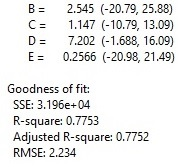
\includegraphics[scale=1.1]{figure/MagicFormulaFrontBagsFitnumbers}
		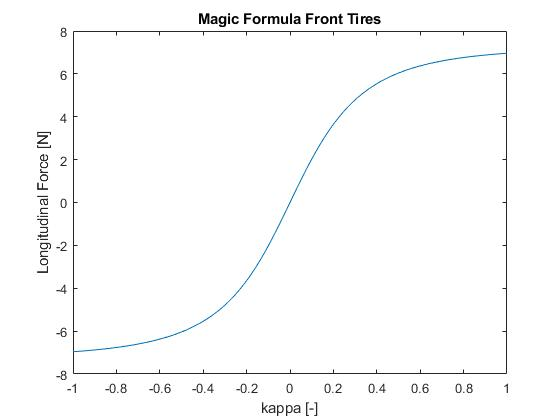
\includegraphics[scale=0.4]{figure/MagicFormulaFrontBagsPic}
        \caption{The front wheels}
    \label{fig:mffront}
\end{subfigure}
	\begin{subfigure}{1\linewidth}
		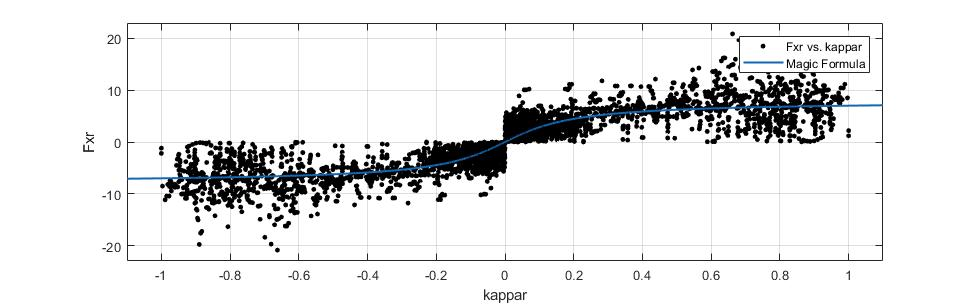
\includegraphics[scale=0.52]{figure/MagicFormulaRearBags}
		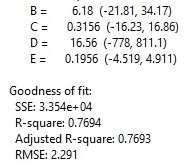
\includegraphics[scale=1.1]{figure/MagicFormulaRearBagsFitnumbers}
		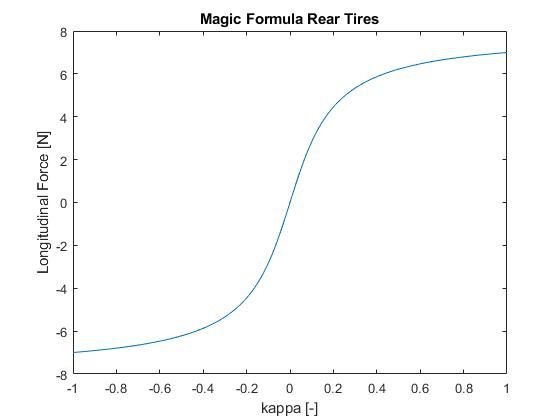
\includegraphics[scale=0.4]{figure/MagicFormulaRearBagsPic}
		
        \caption{The rear wheels}
        \label{fig:mfrear}
    \end{subfigure}
    \caption{Fitted Magic Formula's from combined data}
    \label{fig:mf}
\end{figure*}
\begin{figure}
	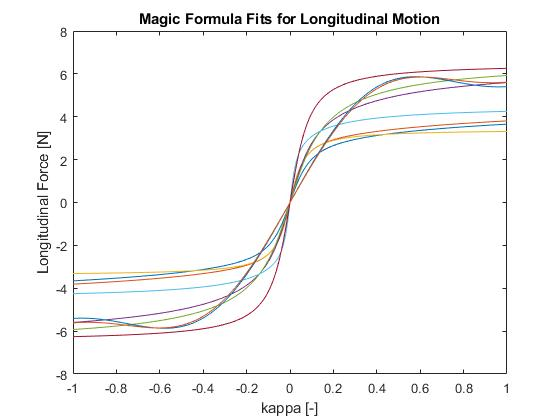
\includegraphics[scale=0.4]{figure/SeperateBags.jpg}
    \caption{Fitted Magic formulas for separate tests}
    \label{fig:MagicFormulaSplit}
\end{figure}
As noticeable from the plots, the Magic Formula does not take its regular form. Even though there are comparisons with the Magic Formula, it still is not what was expected. First of all, the Magic Formula has a peak and descends afterwards. This is not the case with Figures \ref{fig:mf}\subref{fig:mffront} and \ref{fig:mf}\subref{fig:mfrear}. Secondly, most magic formulas ascend much faster than our Magic Formula. 
	There are a few possibilities why our Magic Formula differs from others. First of all, the peak in the Magic Formula (Figure \ref{fig:MagicFit}) is related to tire stiffness. As the tire stiffness increases the peak decreases \cite{Jonson}. As our plastic rims with grip tape approach infinite stiffness when compared to air inflated tires, this peak is very small or does not exist. 
    
A second possibility can be the data given by the Tachometers. The sampling time of ROS is much faster than the sampling time of the Hall sensors. This results in many data points where no revolution is detected. Therefore, this data contains a lot of zeros.  Because of this, interpolation between non-zero values is needed. This can result in inaccurate data.
    
Another possible reason  can be varying tire conditions. Through the process of experimenting, wear definitely occurred. Also heat can have effect on the behavior of these tires. Therefore it is possible that the changing tire conditions led to a less accurate Magic Formula. 
The last possibility can be due to noise generated by the IMU. Looking at figures \ref{fig:mf}\subref{fig:mffront} and \ref{fig:mf}\subref{fig:mfrear} we see a lot of noise in our plots, even with the help of the filters that were used. There are three possible contributions to this noise. First is the RC car we used. As the first aim was to improve the data acquisition software, not much was changed about the car itself. It was not after much testing was done before it became clear that the wheels were not balanced very well. This resulted in many vibrations. Especially the IMU (Inertial Measurement Unit) generated much noise because of this. The second possible explanation is that the IMU has not been properly calibrated. This has proven to be very difficult due to the complexity of the code of the IMU. Lastly, the IMU could not be installed perfectly normal to the floor.

However, the goodness of the fits for the combined experiments of the front and rear tires are decent, around 0.77. Goodness of fit becomes even higher when fitting the Magic Formula for some separate tests, varying between 0.80 and 0.93. The most plausible explanation for the difference between the plots in Figure \ref{fig:MagicFormulaSplit} is that the condition of the tires varies between measurements. Also, the shapes of our plots show comparison with the Magic Formula. This suggests that determining tire characteristics with the help of this experimental setup is heading towards the good direction. With some adjustments, this method can be very useful for determining tire characteristics.

Finally, the magic formula for the slip angles are missing. This is because the dynamixel was not functioning properly. Therefore, the steering angles could not be determined accurately enough to generate proper data. However, if the dynamixel is installed correctly and proper data is generated, it should be easy to determine the magic formula for the slip angles with the method described in this paper.


\section{Conclusion}
The experiments have provided decent data from which the tire characteristics in longitudinal motion could be derived. The IMU has proven to be a great improvement to the project and even though its test results are noisy, they provide a very good insight in the speed and acceleration of the car. From this data, together with the hall-effect sensor data and the used models, a tire model is designed that sufficiently represents the tire characteristics in the longitudinal motion of the car. 
	Even though there is still much room for improvement, this method for determining tire characteristics has proven to be promising. With adjustments that will be discussed in Section 6, a valid representation of the tire characteristics can be made, which could be even closer to reality than currently calculated.
\section{Recommendations}
As seen in previous sections decent results were already accomplished, however many possibilities for improvements are readily found and much more can be done in this area. First of all, many physical improvements could be made to the testbed. Moreover, the signal analysis part of this research could be improved. Last, further steps can be taken towards implementation of this research into autonomous or assisting driver system.

\subsection{Testbed}
As mentioned previously, the current testbed leaves room for improvement. The car is showing signs of wear and multiple impact related accidents have taken its toll on the frame. As it is, the frame is now warped and requires an offset on the front wheels to drive straight again at lower power ranges. However, when driving in the high power ranges the vehicle dynamics become different and the offset will eventually make the car turn. Although this offset can be corrected in the measurements, the fact that it is necessary suggests there are other problems with the data being generated.

Moreover, the measurements are affected by vibrations. To fit the testbed to the Bicycle Model, the original suspension has been replaced by stiff turnbuckle rods, that do not dampen any vibrations of the car. The IMU, unfortunately, is highly susceptible to this noise. Reducing vibrations should be high on the priority list when attempting to improve the results of this research.

Finally, the 3D-printed wheels are hard to balance as the tolerance on the construction method is quite high. As a result of this, the car shows excessive vibrations during tests. This is further enlarged by placing the magnets which may have even higher tolerances. Some effort to improve results might be aimed towards building proper balanced wheels using more precise techniques as a lathe, wheel balancing tools and maybe even custom magnets.

\subsection{Signal analysis}
Another area of improvement is the signal analysis. During this research an attempt was made to convert the signal of the IMU into the Fourier spectrum. However, it was difficult to distinguish the spectrum of noise from the actual signal. Therefore, a filter was created with a cut-off frequency of 5 Hz. It was determined that vibrations from the wheels would be generated from 5.5 Hz onwards and therefore the 5 Hz cut-off frequency was applied. Further signal analysis might improve on this rudimentary constructed filter. When combined with noise reduction, the signal might be cleaned up significantly to give a more clear Fourier spectrum on the noise and the actual signal. By this, a reduced filter can be designed, which might generate a better picture through more data points.  
\subsection{Implementation}
Finally, we look at implementation. The eventual aim of this research is to be able to use it in Nonlinear Model Predictive Control and eventually implementation into cars. However, when looking towards the future it is evident a couple of problems will arise. The first problem with a tire model is that it is heavily dependent on more variables than initially taken into account in this research. A quick grasp would be environment variables like temperature, terrain and humidity. Although these might be determined by adding more sensors to the vehicle, there are also variables which are more difficult to determine. A way of determining the model at any given instant of time might be a more viable approach. This raises new problems though. To determine data points throughout the entire spectrum, the car needs to gather data at high slip ratios at that given time. This is something which can not always be done easily. Further research into generating a model without a lot of especially high slip ratio data points needs to be done to make this possible.
\section{Acknowledgements}

We would like to thank Tam{\'a}s Keviczky and Will van Geest for their supervision, help and their feedback during this entire project. Special thanks go to Will for being always available to us to share his knowledge and expertise in the field of hardware and programming. We would also like to thank Barys Shyrokau for his advice on the models we used for the dynamics and the tire characteristics of the car.
\begin{thebibliography}{9}

% \bibitem{lamport94}
%   Leslie Lamport,
%   {LaTeX: a document preparation system},
%   Addison Wesley, Massachusetts,
%   2nd edition,
%   1994.

\bibitem{NHTSA}
  NHTSA. (2017).
\textit{2016 Fatal Motor Vehicle Crashes: Overview}.
  Retrieved from https://crashstats.nhtsa.dot.gov/Api/Public/Publication/812456.


\bibitem{Tamas}
 Keviczky, T. Falcone, P. Borrelli, F. Asgari, J. Hrovat, D. (2006).
\textit{Predictive Control Approach to Autonomous Vehicle Steering}.
American Control Conference, Minneapolis, Minnesota, June 14-16, pp. 4670-4675.


\bibitem{Jonson}
Jonson, A. Olsson, E. (2016).
\textit{A Methodology for Identification of
Magic Formula Tire Model Parameters
from In-Vehicle Measurements} (Master's Thesis, Chalmers University of Technology, Gothenburg, Sweden). 


\bibitem{Liu}
Liu, G. Ren, H. Chen, S, Wenzhu, W. (2014).
\textit{The 3-DoF bicycle model with the simplified piecewise linear tire model}.
International Conference on Mechatronic Sciences, Electric Engineering and Computer (MEC).


\bibitem{Pacejka}
Pacejka, H.B. (2012).
\textit{Tyre and Vehicle Dynamics}.
Butterworth-Heinemann, Apr. 


\bibitem{uil}
UIL R.T. (2007).
\textit{Tyre models for steady-state vehicle handling analysis}.
  
  
\bibitem{IMUfilter}
Valenti, G.R. Dryanovski, I. Xiao, J. (2015).
\textit{Keeping a Good Attitude: A Quaternion-Based Orientation Filter for IMUs and MARGs}.
Sensors 2015, 15(8), 19302-19330
City college of New York, New York.









 


\end{thebibliography}



%%%%%%%%%%%%%%%%%%%%%%%%%%%%%%%%%%%%%%%%%%%%%%%%%%%%%%%%%%%%%%%%%%%%%%






\end{document}